\chapter{Measurement set-up: overview}
\label{app:setupoverview}
\setheader{Measurement set-up: overview}

In this appendix an overview of the measurement set-up will be given for replication.
The measurements were conducted in the anechoic room in the Physics department at the Delft University of Technology.
The used software to generate the TSP and MLS sequences is made by Thomas \cite{Thomas2006}.
First the used hardware and the connection between those will be addressed, after that the measurement procedure will be repeated in short and at the end of this appendix some pictures of the measurement set-up are given.

\section{Used hardware}
\begin{itemize}
\item[]\textbf{Smartphone and measurement microphone}
\item \nexus, with an application specifically made for this project (which implementation is detailed in \cite{BAP:RoySjoerd});
\item Microphone: Br\"uel \& Kj\ae r Free-field microphone \cite{manual:microphone} (Figure \ref{fig:app:hardware:mic});
\item WiFi-router to connect the smartphone to the computer;
\item[]\textbf{Set-up hardware}
\item Aluminium arc, with a radius of 1.21 meter, with a reach of angles in $[-75,75]^\circ$, were the reference $0^\circ$ is the horizon, or equivalently $(\phi\in[15,165]^\circ)$;
\item Turntable: the turntable which is part of the remote controllable Br\"uel \& Kj\ae r 9640 turntable system \cite{manual:turntable};
\item A stick, with a length of 1.15 m, which fits in the turntable, with enough surface at the top to support the smartphone, which top was covered with sound absorbing foam;
\item A stick, with a length of 1.15 m, which fits in the turntable, with $290\times240\times8$ mm plywood plate on top;
\item Double-sided tape (1 mm thick);
\item Tripod;
\item[]\textbf{Acoustic system}
\item HP EliteBook 8540w personal computer with Windows 8 operating system, running \matlab Student R2014a;
\item RME Fireface 800 \cite{manual:fireface};
\item Audio amplifier: a custom-build 8-channels amplifier of 25W per channel with $4\Omega$, built with the IC Philips TDA8560Q;
\item Loudspeaker: Tymphany 4"Midrange loudspeaker, type number M10MD-39-08 \cite{manual:loudspeaker} (Figure \ref{fig:app:hardware:loudspeaker});
\item[]\textbf{Connections}
\item Firewire cable to connect the computer to the Fireface;
\item XLR-cable to connect the Fireface to the audio amplifier;
\item Twist-lock Speaker cable to female-banana and banana cable to connect the amplifier to the loudspeaker;
\item Coaxial cable, RCA cable and a connection between these two, to connect the measurement microphone to the Fireface.
\end{itemize}

\section{Volume settings}
Before the start of the measurements the settings of the equipment have to be adjusted such that:
\begin{itemize}
\item The Fireface does not clip (its GUI is very clear about clipping), this can be done in two ways:
\begin{itemize}
\item Turning the volume down in Windows 8 (our settings: 5\% volume);
\item Using a gain factor in {\matlab} to lower the outputsignal (our settings: -7 dB).
\end{itemize}
\item The loudspeaker signal is not too loud so it is distorted by the loudspeaker or the loudspeaker is affected by the signal, this can be done in two ways:
\begin{itemize}
\item Changing the volume settings of Windows 8 and \matlab;
\item Changing the volume settings of the Fireface in its GUI (our settings: -30 dB outputsignal).
\end{itemize}
\end{itemize}

\section{Conducting the measurements}
The measurements are conducted with a $9^\circ$ equiangular sampling scheme as described in Section \ref{ssec:equiangular}.
For measurements in mid-air, the smartphone was placed on the stick covered with foam.
For measurements $\phi\leq90^\circ$ the smartphone lay on its back, with its middle point in the middle of the stick, starting with the speechside toward the loudspeaker and the turntable was turned in positive direction in \matlab~(negative direction according to the turntable system).
First all 41 measurements with the TSP sequence where conducted, where after the MLS sequences was used to measure.
For measurements $\phi>90^\circ$ the smartphone was flipped over so it laid on its screen, and the turntable was instructed to turn in the other direction, so the the movement of the microphone with respect to the speaker is the same as for the measurements $\phi\geq90^\circ$.

For angles $\phi \in[0,15\rangle\cup\langle165,180]^\circ$ the turntable was positioned in an angle and raised to place the phone in the same position in space.
For stability the smartphone was taped to the stick with double-sided tape.

The measurements with the phone placed on a surface were conducted using the stick, with the plywood attached to it.
These were only measured for $\phi\in[0,135]^\circ$, once with the screen on the surface (face down) and once with the back of the phone on the surface (face up). For $\phi \in[0,15\rangle$ also the double-sided tape is used.
For these measurements the turntable always turned in positive direction following the \matlab-code.

\subsection{Measurements with the microphone}
For equalization these measurements were also conducted with the B\&K microphone.
The microphone was placed on a tripod on top of the turntable, also with a distance of 1 meter from the loudspeaker (positioned at $\phi=90^\circ$), and the same code as used for the smartphone measurements was run, except the control-functionality of the turntable was turned off, so the microphone stayed in the same place.

\vspace{0.5in}

Pictures of the measurement set-up can be found on the next page.

\clearpage
\section{Pictures}
\invisiblesection{Pictures}

\begin{figure}[h!]
        \centering

        \begin{subfigure}[b]{0.33\textwidth}
                \centering
    			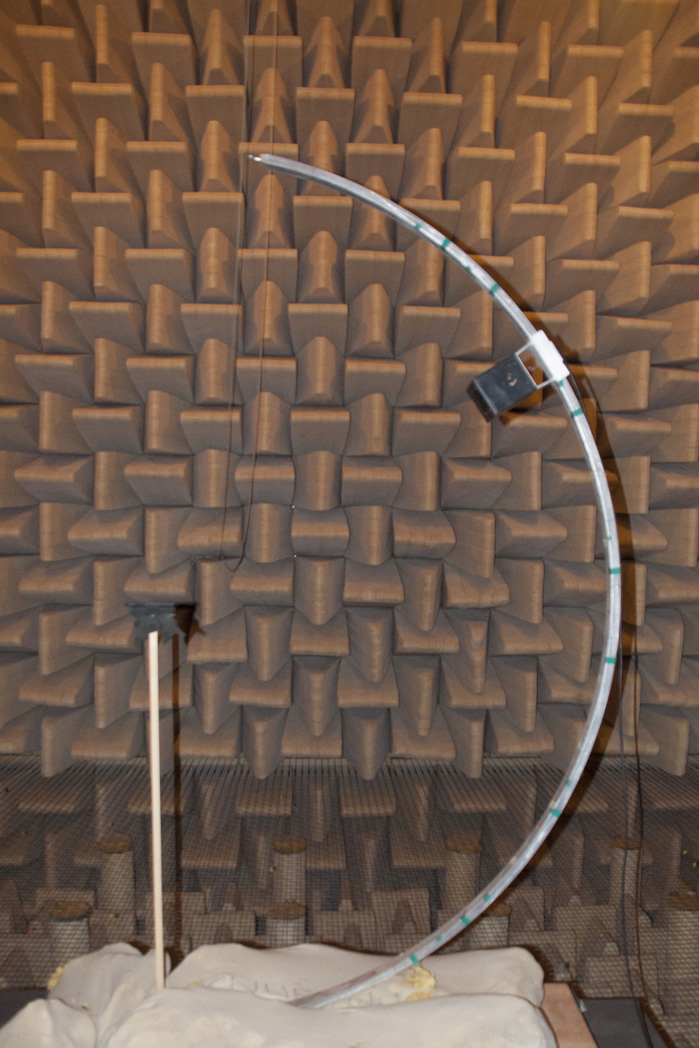
\includegraphics[height=0.28\textheight]{cover/onzecover.jpg}
    			\caption{Measurement at $\phi=63^\circ$}
			    \label{fig:phi=63}
        \end{subfigure}~
        \begin{subfigure}[b]{0.33\textwidth}
			    \centering
    			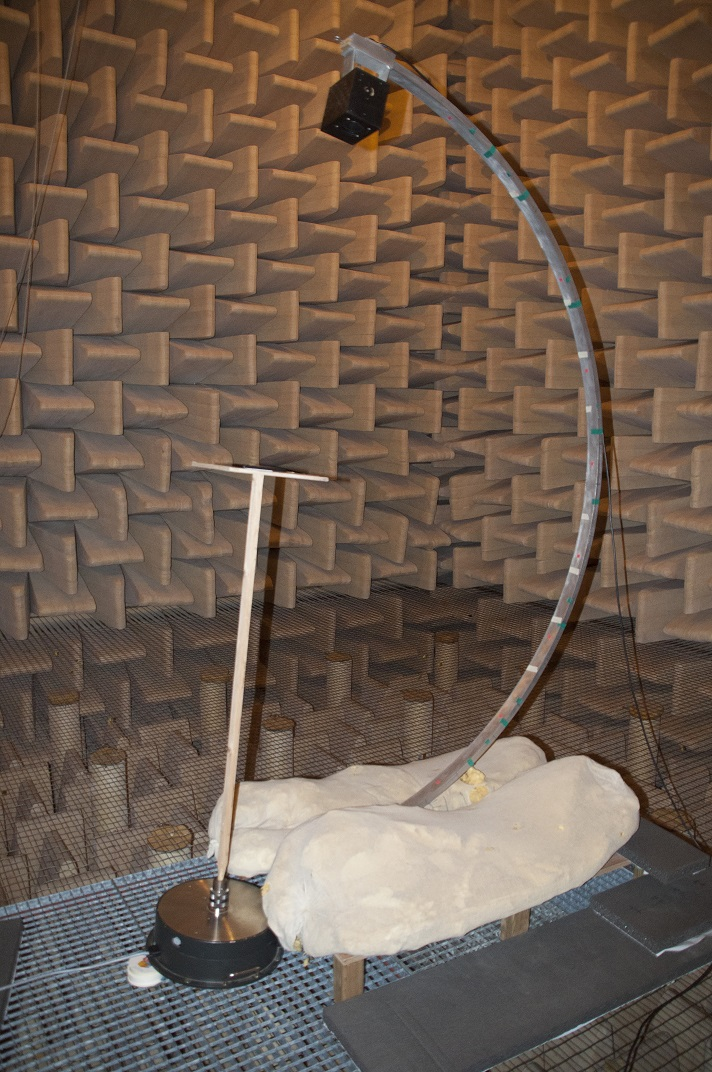
\includegraphics[height=0.28\textheight]{afbeeldingen/opstelling_schuin.jpg}
    			\caption{Measurement at $\phi=9^\circ$}
			    \label{fig:phi=9}
                
        \end{subfigure}~
        \begin{subfigure}[b]{0.33\textwidth}
			    
                \centering
    			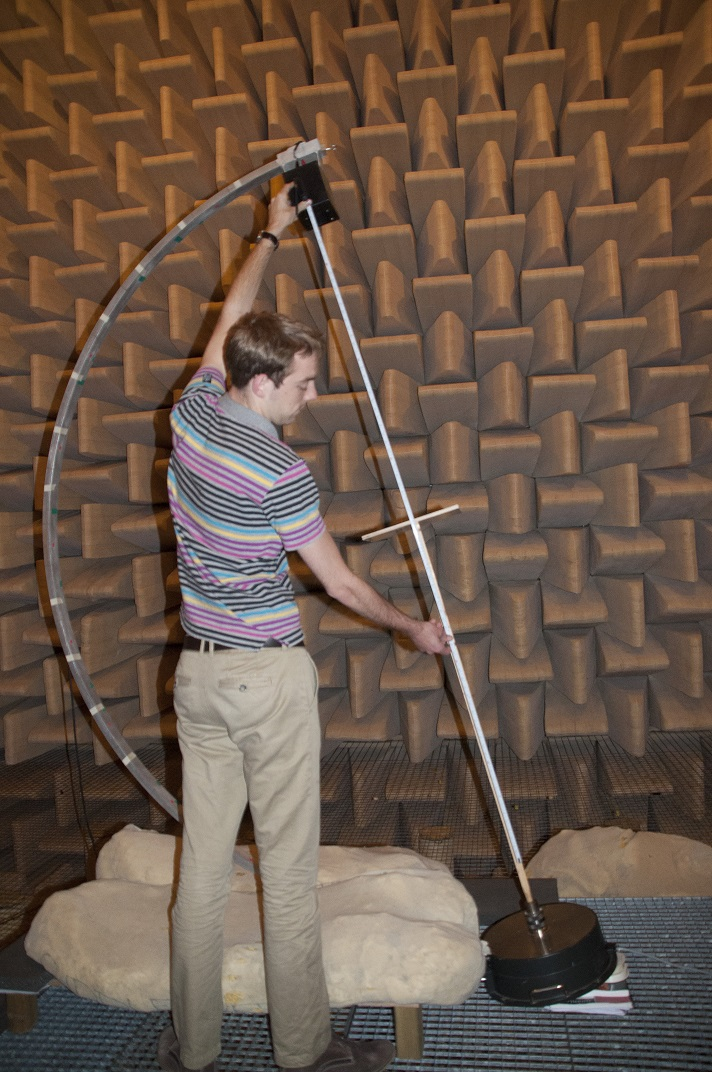
\includegraphics[height=0.28\textheight]{afbeeldingen/tim.jpg}
    			\caption{Measurement at $\phi=0^\circ$}
			    \label{fig:tim}
        \end{subfigure}
        
        \begin{subfigure}[b]{0.5\textwidth}
			    
                \centering
    			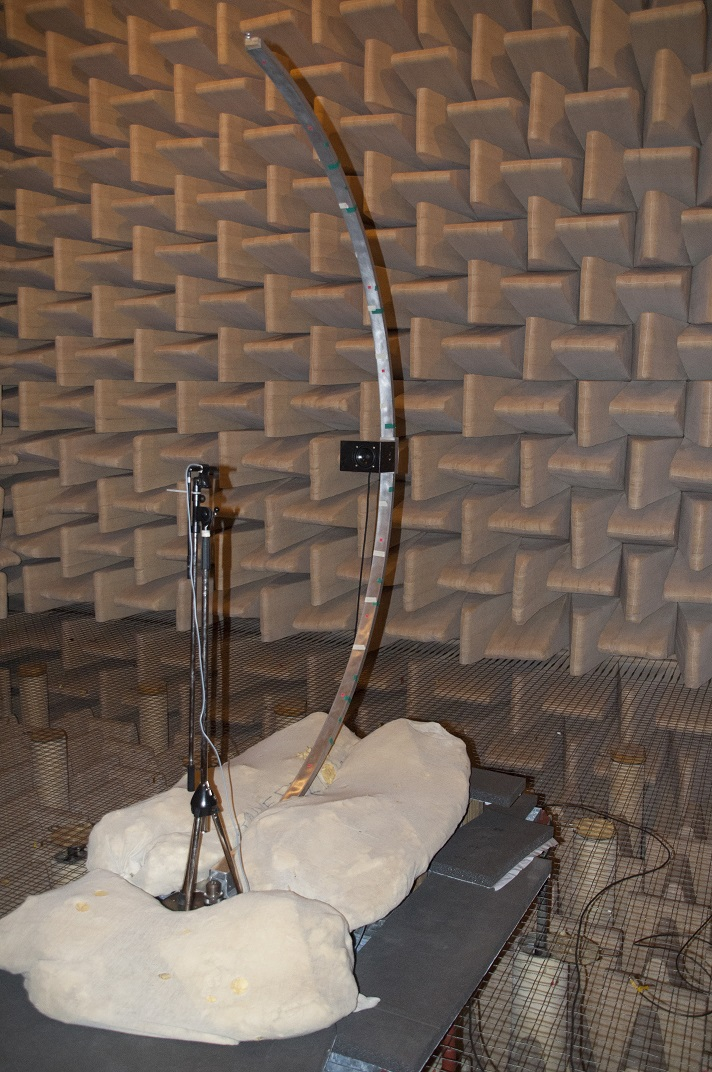
\includegraphics[height=0.28\textheight]{afbeeldingen/meetmic.jpg}
    			\caption{Measurement with the B\&K microphone}
			    \label{fig:meetmic}
        \end{subfigure}~
        \begin{subfigure}[b]{0.5\textwidth}
			    
                \centering
    			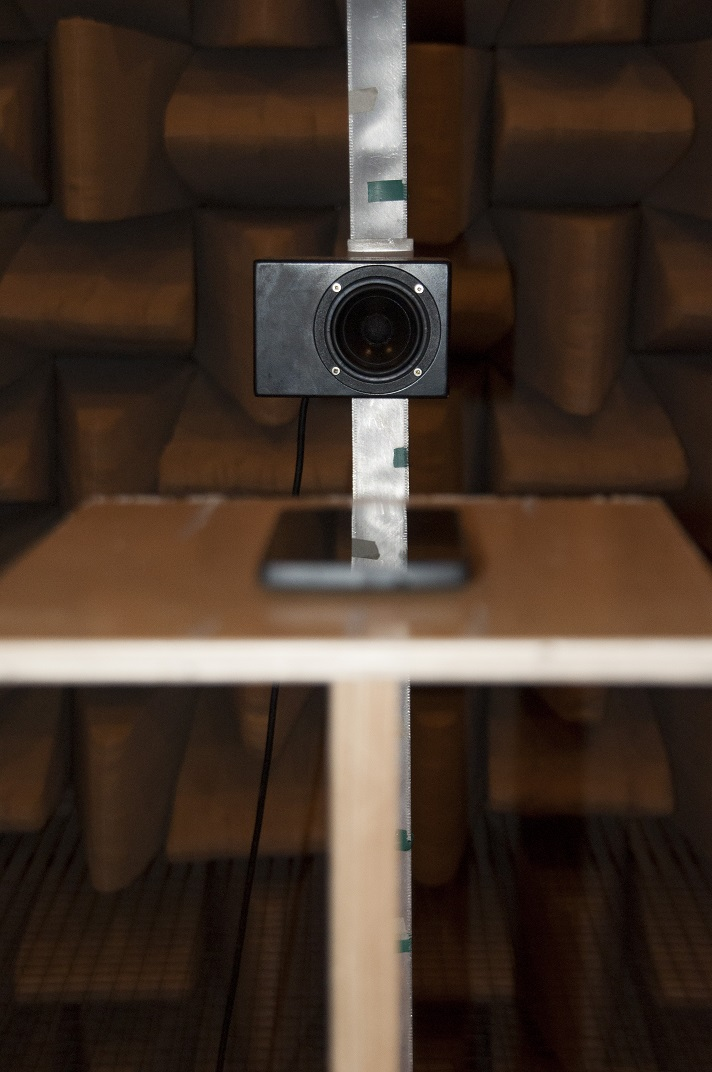
\includegraphics[height=0.28\textheight]{afbeeldingen/plywood.jpg}
    			\caption{Measurement at $\phi=90^\circ$, face up on the surface}
			    \label{fig:phi=90FU}
        \end{subfigure}
        
        \begin{subfigure}[b]{0.5\textwidth}
			    \centering
    			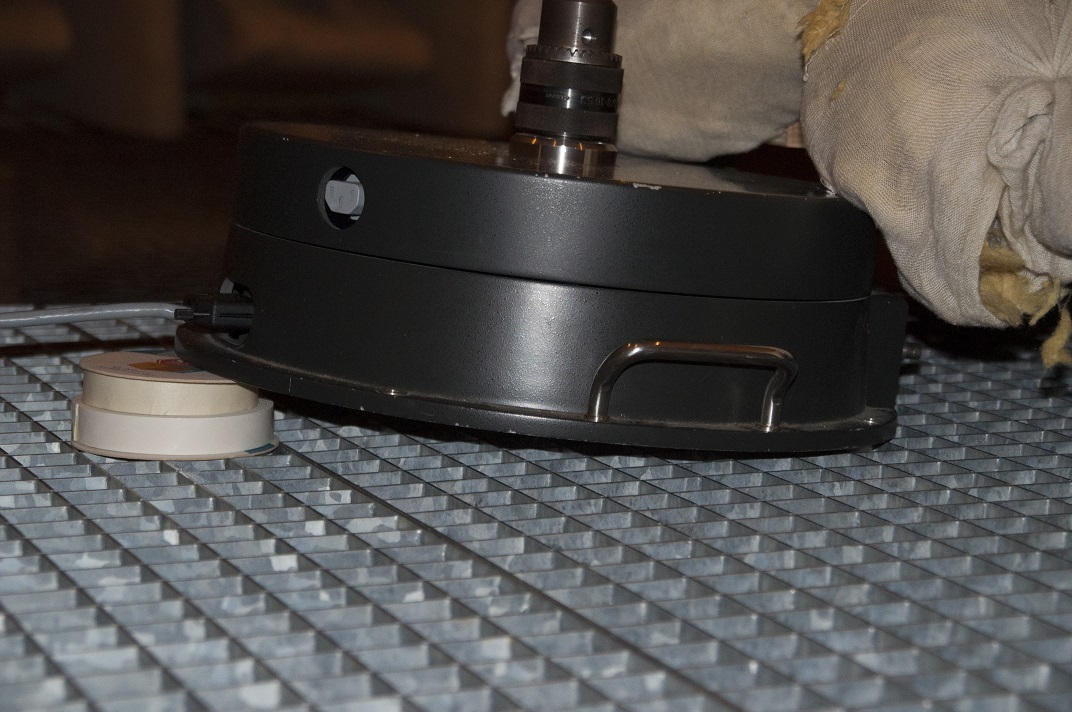
\includegraphics[width=\textwidth]{afbeeldingen/turntable_schuin.jpg}
    			\caption{Placement of turntable an an angle of $6^\circ$}
			    \label{fig:turnt_schuin}
                
        \end{subfigure}~
        \begin{subfigure}[b]{0.5\textwidth}
			    \centering
    			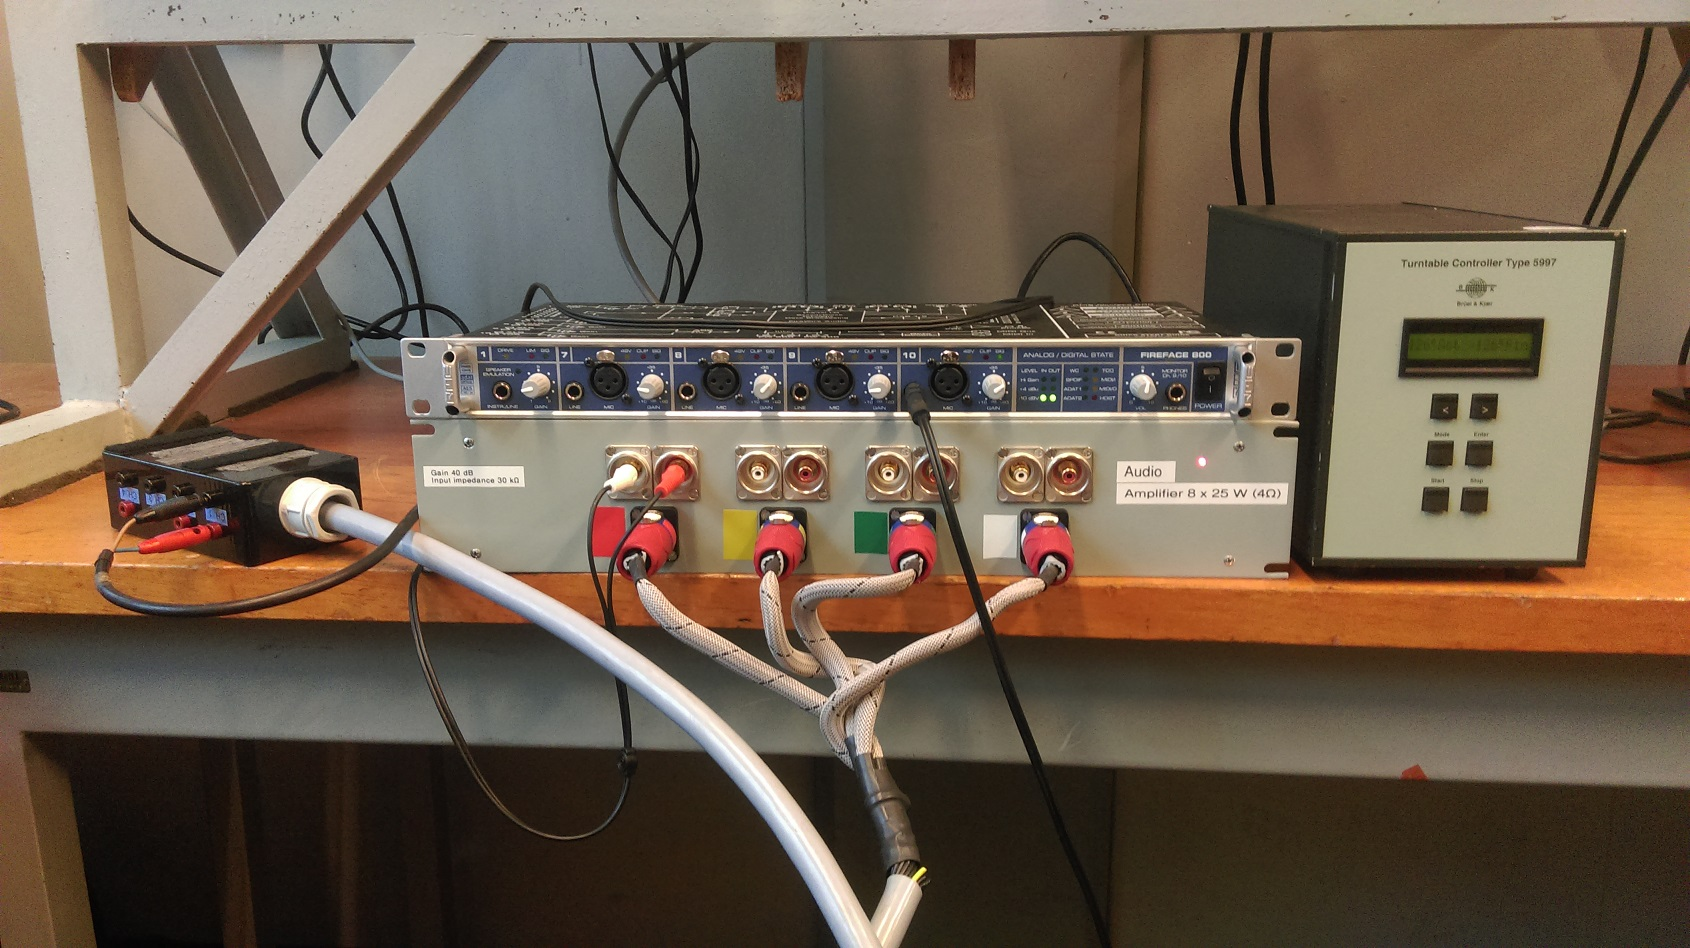
\includegraphics[width=\textwidth]{afbeeldingen/hardware.jpg}
    			\caption{Connection between the hardware}
			    \label{fig:hardware}
                
        \end{subfigure}
        
        \caption[Measurement set-up overview]{Pictures of the measurement set-up}
        \label{fig:app:overview}
\end{figure}